\documentclass{article}
\usepackage{setspace}
\usepackage{amsfonts}
\usepackage{graphicx}
\usepackage{amsmath}
\graphicspath{{./figures/}}

\title{Heterogeneous multiscale modeling of plasma confined to a two-dimensional periodic domain}
\author{Jeffrey Haack, Michael Murillo, Jacob Price, Gil Shohet}


\begin{document}

\maketitle

\begin{abstract}
Plasma modeling can be conducted with varying levels of detail. The Bhatnagar-Gross-Krook approximation is an effective kinetic model for hot plasma given an accurate relaxation parameter. This parameter, however, is difficult to know \emph{a priori}. Molecular dynamics offers a fully detailed model for ionic motion. The heterogeneous multiscale method (HMM) provides a computational and analytical link between disparate physical models. In this paper, we present a proof of concept of HMM as a modeling method for hot plasma. The unknown relaxation parameter can be computed from short molecular simulations, and then used in subsequent kinetic time steps. Simulations using the hybrid kinetic-molecular dynamic model are both more accurate than the kinetic model alone, and orders of magnitude more efficient than the molecular dynamics model alone. The HMM philosophy can be used similarly to hybridize physical models in a way that creates a stark improvement over both original models.
\end{abstract}

\section{Introduction}

Many mathematical and scientific problems contain phenomena at widely different scales. Multiscale modeling aims to take advantage of this disparity to understand complex behavior at each level of detail \cite{weinan2011principles}. Multiphysics problems are a prototypical example of problems that are well-addressed by a multiscale approach. There is a hierarchy of physical models of varying levels of detail and coarseness. Quantum mechanics (QM) provides a complete description of physical interactions, but is often computationally and analytically intractable for all but the simplest systems. From quantum mechanics, one can derive laws of molecular dynamics (MD) as a more tractable, but less detailed physical description than the wave functions of QM. From MD, kinetic theory (KT) can be derived as a statistical description of molecular motion. An even coarser model, hydrodynamics, can be derived either directly from MD or from KT.

With each step up in the hierarchy, physical detail is sacrificed for intuition and computational tractability. In reality, these levels of detail form a continuum, rather than classes of problems. Hydrodynamics describe bulk motion well, unless that motion involves a crack in the material, or a propagating shock. In these regions of interest, kinetic effects, or even molecular effects cannot be disregarded. In this way, multiphysics and multiscale modeling become important in different regions of interest.

Often coarser models contain parameters that can be interpreted as averaged quantities from higher detail models. For example, stress tensors in hydrodynamics can be computed from the second velocity moment of a kinetic description of the same system. When one confines oneself to a coarse model, these parameters can prove difficult. These parameters are precomputed as a function of macroscopic variables and tabulated in a reference table for use in all later simulations. One major limitation is the fact that we may be unable to anticipate all relevant arrangements. It would be better to be able to compute these parameters accurately ``on the fly.''

This leads to the concept of the heterogeneous multiscale method (HMM) \cite{weinan2007heterogeneous}. HMM takes a top-down approach to multiphysics modeling. Two (or more) levels of physical detail are selected, such that the analysis and computation could be completed in any level and yield consistent results. HMM focuses on the coarsest model, as this is one can be computed efficiently over a much larger time scale than the more detailed model. This coarse model, as discussed above, contains parameters that are averaged quantities from the higher-detail model. The general approach is to spend most computational time in the coarse regime, periodically down sampling to the fine regime to use brief simulations to recompute parameters used in the coarse regime. The result is a hybrid simulation method that contains the computational speed of the coarse model with highly accurate parameters drawn from the fine model. The proposed method is illustrated in Figure \ref{HMM}.



\begin{figure}[h]\begin{center}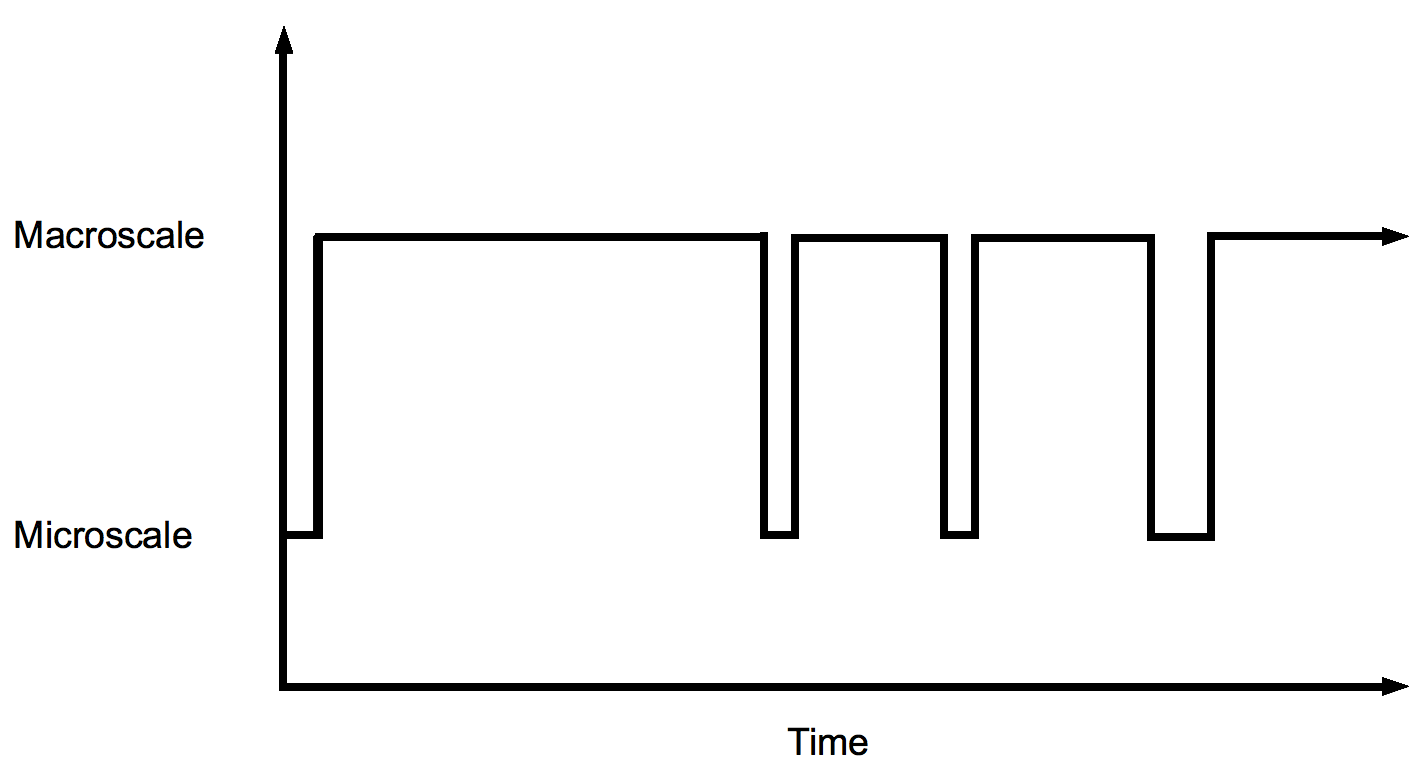
\includegraphics[width=.6\linewidth]{scheme.pdf}\caption{A cartoon of the computational time spent in different computational regimes during an HMM simulation.}\label{HMM}\end{center}\end{figure}

The structure of this paper will be as follows. In Section 2, we will describe the system of interest and the selected physical regimes, along with their governing equations. In Section 3, we rigorously connect the fine grain description to the coarse grain description, and in doing so demonstrate the exact nature of the connecting parameters. We also rigorously rationalize simplifying decisions made in the modeling steps. In section 4, we make explicit the manner in which we transition between levels of detail. In practice, this is the most difficult part of HMM. In Section 5, we non-dimensionalize both models to isolate interesting timescales and improve numerical computations. In Section 6, we present the results of our computations, comparing fully fine-grained simulations with hybrid HMM simulations. We comment on insights that can be gleaned from the longer time scale the HMM method allows us to study. Finally, in Section 7, we comment on the possibilities and downsides of this scheme for this specific problem and similar classes of problems.

\section{Plasma modeling}

Plasma is a dense, electrically neutral system of electrons and multiple species of charged ions, in which each ion interacts with many neighbors, making collective effects critical \cite{sturrock1994plasma}. This near-neighbor interaction is represented by the \emph{Debye length} $\lambda$. Because opposite charges attract, each positive ion tends to be surrounded by several negatively charged electrons, which effectively ``screen'' the electrostatic field due to the other particles. Plasma particles only significantly interact with other particles within one Debye length. Other interactions drop off due to the strong length dependence on forces, and an effective ``screening'' by background electrons. Examples of plasmas include astrophysical phenomena such as stars and the interplanetary medium, terrestrial phenomena such as lightning and aurorae, and technological constructs such as plasma televisions and material used in fusion reactor research.

Our system of interest is hot plasma in which the ions are confined to a two-dimensional plane on a periodic domain. Periodic boundary conditions effectively represent the behavior of a much larger domain, since particle interactions are screened by the Debye length. Particles are only affected by their nearest neighbors. One reason we confine ourselves to two-dimensional simulation is computational efficiency. We seek to demonstrate multiscale plasma modeling through a proof of concept. All of the conclusions and methods described in this paper can be extended to more complicated systems with little difficulty. Additionally, there are physical examples of plasmas that are confined to a plane. \emph{Dusty plasmas} consist of large (millimeter to nanometer), charged particles. They can be found in the mesosphere of the earth, industrial processing, and laboratory experiments. In experiments, they can be confined to a plane by a balance of gravitational force and electric force from a vertical lab-generated electric field. Electrons, which weigh far less than the ions, are free to move in three dimensions, but the motion of the ions is confined to a flat plane \cite{shukla2001introduction}.

In order to use HMM to simulate this system, we select the Bhatnagar-Gross-Krook (BGK) approximation of the Boltzmann equation of kinetic theory as our coarse model and molecular dynamics as our fine model. The quantity of interest in the BGK model is the distribution of each ion species. For ion species $k$, we represent this distribution by $f_k(\mathbf{r},\mathbf{p})$, the distribution of particles at position $\mathbf{r}=(x,y)$ with momentum $\mathbf{p}=(p_x,p_y)$. The partial differential equation governing this distribution is
\begin{equation}
\begin{split}
&\frac{\partial f_k}{\partial t}+\mathbf{v}\cdot\nabla_\mathbf{r}f_k+\frac{Z_ke}{m_k}E\cdot\nabla_\mathbf{v}f_k=\sum_l\frac{f_{kl}^{eq}-f_k}{\tau_{kl}}\\
&E(\mathbf{r},t)=-\int\frac{e}{4\pi\epsilon_0}\rho(\mathbf{r}',t)\nabla_\mathbf{r}\left(\frac{e^{-|\mathbf{r}-\mathbf{r}'|/\lambda}}{|\mathbf{r}-\mathbf{r}'|}\right)\,d\mathbf{r}'\\
&f_k(\mathbf{r},\mathbf{v},0)=f_{k}(\mathbf{r},\mathbf{v})\\
&\left.f_k(\mathbf{r},\mathbf{v},t)\right|_{x=0}=\left.f_{k}(\mathbf{r},\mathbf{v},t)\right|_{x=L_x},\;\;\;\;
\left.f_k(\mathbf{r},\mathbf{v},t)\right|_{y=0}=\left.f_{k}(\mathbf{r},\mathbf{v},t)\right|_{y=L_y}\\
\end{split}
\label{eq:BGK}
\end{equation}Here, $Z_k$ is the charge of the ion and $m_k$ is its mass. $E(\mathbf{r})$ is the electric field at position $\mathbf{r}$ due to all the ions of all species in the system. In its expression, $e$ is the unit charge, $\epsilon_0$ is the vacuum permittivity, and $\lambda$ is the Debye length determining the degree of electron screening. $f_{kl}^{eq}$ is the equilibrium distribution of the mixture of ion species $k$ and $l$, and $\tau_{kl}$ is a relaxation time for this equilibrium. An identical partial differential equation exists for every species of ion, simply replacing every $k$ with $i$ for species $i$, and so on.

In the fine MD model, we have $n$ ions that are individually tracked according to the Hamiltonian equations
\begin{equation}
\begin{split}
\frac{\partial \mathbf{r}_i}{\partial t}&=\frac{1}{m_i}\nabla_{\mathbf{v}_i} H\\
\frac{\partial \mathbf{v}_i}{\partial t}&=-\frac{1}{m_i}\nabla_{\mathbf{r}_i}H\\
H(\{\mathbf{r}_k\}_{k=1}^N,\{\mathbf{v}_k\}_{k=1}^N)&=\sum_\alpha\left[\frac{m_\alpha|\mathbf{v}_\alpha|^2}{2}+\sum_{\alpha<j}U_{\alpha j}(\mathbf{r}_\alpha,\mathbf{r}_j)\right].
\end{split}\label{eq:MD}
\end{equation}Here $\mathbf{r}_i$ and $\mathbf{v}_i$ are the position and velocity of ion $i$. Consider $\Omega$ different species with their own charges and masses. $H$ is the Hamiltonian of the system, consisting of the sum of the kinetic energy and the potential energy. Ions evolve according to these simple equations in a periodic two-dimensional box. Note that, though motion is confined to this two dimensional box, we assume our system is actually three-dimensional, as in the dusty plasma experiments. Indeed, the electrons are able to move freely in 3D space; only the ions are confined.

The potential energy $U_{ij}(\mathbf{r}_i,\mathbf{r}_j)$ represents the potential energy on particle $i$ due to particle $j$, screened by the electrons. It depends upon the identity of the two particles, as well as their positions. We leave this potential general when deriving the kinetic equations, such that this derivation is generalizable to any desired potential. We only require that the potential satisfy the constraint that $\sum_i\sum_{i<j}U_{ij}(\mathbf{r}_i,\mathbf{r}_j)$ be fixed under a permutation of particle indices. That is,
\[\sum_i\sum_{i<j} U_{ij}(\mathbf{r}_i,\mathbf{r}_j)=\sum_{p(i)}\sum_{p(i)<p(j)}U_{p(i),p(j)}(\mathbf{r}_{p(i)},\mathbf{r}_{p(j)})
\] for all permutations $\{1,2,\dots\}\to\{p(1),p(2),\dots\}$. This simply implies that the total potential energy is independent of the choice of indices, a natural requirement. 

Let the indices of the particles that are of species one be expressed as $S_1=\{1,\dots, N_1\}$ where $N_1$ is the number of ions of species one. Similarly, the indices of species $k$ are $S_k=\{1+\sum_{l=1}^{k-1} N_l,\dots,\sum_{l=1}^kN_l\}$. Ions of species $k$ have mass $m_k$ and charge $Z_k$. Note that the total number of ions $N=\sum_{k=1}^\Omega N_k$. Interparticle potentials can be written as $U_{ij}(\mathbf{r}_i,\mathbf{r}_j)=U_{\{kl\}}(\mathbf{r}_i,\mathbf{r}_j)$ where $i\in S_k$ and $j\in S_l$. In this paper, we use the Yukawa potential to simulate electron screening. the potential energy between two ions at position $\mathbf{r}$ and $\mathbf{r}'$ with charges $Z_k$ and $Z_l$ respectively is
\begin{equation}U_{\{kl\}}(\mathbf{r},\mathbf{r}')=\frac{Z_kZ_le^2}{4\pi\epsilon_0}\frac{e^{-|\mathbf{r}-\mathbf{r}'|/\lambda}}{|\mathbf{r}-\mathbf{r}'|}.\label{eq:yukawa}
\end{equation}
A fully detailed description in this regime would include the Hamiltonian equations for the motion of the electrons, however for simplicity we do not track the electrons individually. We only monitor their collective effects on each ion.

\section{Multiphysics connection}
Our system is described in full detail when we evolve every ion in the molecular dynamics simulation according to the Hamiltonian equations (\ref{eq:MD}). We will derive, from this starting point, the BGK kinetic theory formulation of the problem (\ref{eq:BGK}). We construct an Klimontovich distribution \cite{klimontovich1983kinetic} $\phi_k$ for each species $k$ that stores the location $\mathbf{r}_i$ and momentum $\mathbf{p}_i$ of every ion of that species at a given time $t$:
\begin{equation}\phi_k(\mathbf{r},\mathbf{v},\{\mathbf{r}_\alpha\}_{\alpha=1}^{N},\{\mathbf{v}_\alpha\}_{\alpha=1}^{N},t)=\sum_{i\in S_k}\delta\left(\mathbf{r}-\mathbf{r}_i(t)\right)\delta\left(\mathbf{v}-\mathbf{v}_i(t)\right).
\end{equation}$\delta(x)$ is the Dirac delta function. We are interested in the time evolution of these indicator functions. Thus, an aside relating to distributions and their derivatives is warranted

\subsection{Distributional derivatives}
Consider the set of test functions, $D(\mathbb{R})$ that are infinitely differentiable and have compact support. A distribution is a linear mapping $T: D(\mathbb{R})\to\mathbb{R}$. By convention, the operation of a distribution $T$ on a target function $f$ is written $\langle T,f\rangle$. The Dirac delta ``function'' can thus be written $\langle \delta,f\rangle=f(0)$.

The derivative of a distribution is defined as $\langle T',f\rangle=-\langle T,f'\rangle$. This is a consequence of integration by parts:
\begin{eqnarray*}
\langle T',f\rangle=\int_{-\infty}^\infty \delta'(x)f(x)\;dx=\left[f(x)\delta(x)\right]_{-\infty}^\infty-\int_{-\infty}^\infty \delta(x)f'(x)\;dx=-\langle T,f'\rangle
\end{eqnarray*}We discount the first term in the integration by parts because our test functions are considered equal to zero outside of a bounded set. Thus, by this definition, the derivative of the Dirac delta function operating on a function $f$ would simply be:
\[\frac{d}{dx}(\delta(f(x)))=-f'(0).
\]Though we will not explicitly compute this derivative, it suffices to show that it exists and is well-defined. The above definition of the distributional derivative in terms of transferring derivatives from the distribution to the internal function also allows for a seamless use of the product and chain rules in their standard forms in the presence of distributions.  Our problem utilizes two-dimensional Dirac delta functions, defined as
\[\delta(\mathbf{r})=\delta(r_x)\delta(r_y).
\]The gradient of this function similarly exists:
\begin{eqnarray*}
\nabla_\mathbf{r}\delta(\mathbf{r})=\left(\delta(r_y)\frac{d}{dr_x}\delta(r_x),\delta(r_x)\frac{d}{dy}\delta(r_y)\right).
\end{eqnarray*}Gradients of two-dimensional delta functions are thus well defined. We will make use of a useful identity relating to derivatives of delta functions. Recall that the argument of the delta functions used in $N$ took the form $\mathbf{f}=\mathbf{a}-\mathbf{b}$. Consider the Dirac delta gradient with respect to each variable:
\begin{align*}
\nabla_\mathbf{a}\delta(\mathbf{a}-\mathbf{b})&=\left(\delta(a_y-b_y)\langle \delta_{a_x},a_x-b_x\rangle,\delta(a_x-b_x)\langle \delta_{a_y},a_y-b_y\rangle\right)\\
&=\left(-\delta(a_y-b_y)\left\langle\delta,\frac{\partial}{\partial a_x}(a_x-b_x)\right\rangle,-\delta(a_x-b_x)\left\langle\delta,\frac{\partial}{\partial a_y}(a_y-b_y)\right\rangle\right)\\
&=(-\delta(a_y-b_y),-\delta(a_x-b_x))\\
\nabla_\mathbf{b}\delta(\mathbf{a}-\mathbf{b})&=\left(\delta(a_y-b_y)\langle \delta_{b_x},a_x-b_x\rangle,\delta(a_x-b_x)\langle \delta_{b_y},a_y-b_y\rangle\right)\\
&=\left(-\delta(a_y-b_y)\left\langle\delta,\frac{\partial}{\partial b_x}(a_x-b_x)\right\rangle,-\delta(a_x-b_x)\left\langle\delta,\frac{\partial}{\partial b_y}(a_y-b_y)\right\rangle\right)\\
&=(\delta(a_y-b_y),\delta(a_x-b_x))
\end{align*}From this, we see we can make the convenient substitution:
\begin{equation}
\nabla_{\mathbf{r}_i}\delta(\mathbf{r}-\mathbf{r}_i)=-\nabla_\mathbf{r}\delta(\mathbf{r}-\mathbf{r}_i)\label{delderivswitch}
\end{equation}
\subsection{Derivation of BGK}
Returning our attention to the time evolution of the Klimontovich distributions $\phi_k$:
\begin{align*}
\frac{\partial \phi_k}{\partial t}=\sum_{i\in S_k}& \frac{\partial}{\partial t}\left[\delta(\mathbf{r}-\mathbf{r}_i(t))\delta(\mathbf{v}-\mathbf{v}_i(t))\right]\\
=\sum_{i\in S_k}& \delta(\mathbf{v}-\mathbf{v}_i(t))\frac{\partial}{\partial t}\delta(\mathbf{r}-\mathbf{r}_i(t))+\delta(\mathbf{r}-\mathbf{r}_i(t))\frac{\partial }{\partial t}\delta(\mathbf{v}-\mathbf{v}_i(t))\\
=\sum_{i\in S_k}&\bigg\{\delta(\mathbf{v}-\mathbf{v}_i(t))\frac{\partial(\mathbf{r}-\mathbf{r}_i(t))}{\partial t}\cdot\nabla_{(\mathbf{r}-\mathbf{r}_i)}[\delta(\mathbf{r}-\mathbf{r}_i(t))]\\
&+\delta(\mathbf{r}-\mathbf{r}_i(t))\frac{\partial(\mathbf{v}-\mathbf{v}_i(t))}{\partial t}\cdot\nabla_{(\mathbf{v}-\mathbf{v}_i)}[\delta(\mathbf{v}-\mathbf{v}_i(t))]\bigg\}\\
=\sum_{i\in S_k}&\bigg\{\delta(\mathbf{v}-\mathbf{v}_i(t))(-1)\frac{\partial \mathbf{r}_i(t)}{\partial t}\cdot\nabla_{(\mathbf{r}-\mathbf{r}_i)}[\mathbf{r}_i]\cdot\nabla_{\mathbf{r}_i}[\delta(\mathbf{r}-\mathbf{r}_i(t))]\\
&\delta(\mathbf{r}-\mathbf{r}_i(t))(-1)\frac{\partial \mathbf{v}_i(t)}{\partial t}\cdot\nabla_{(\mathbf{v}-\mathbf{v}_i)}[\mathbf{v}_i]\cdot\nabla_{\mathbf{v}_i}[\delta(\mathbf{v}-\mathbf{v}_i(t))]\bigg\}\\
=\sum_{i\in S_k}&\bigg\{\delta(\mathbf{v}-\mathbf{v}_i(t))(-1)\frac{\partial \mathbf{r}_i(t)}{\partial t}(-1)(-1)\cdot\nabla_{\mathbf{r}}[\delta(\mathbf{r}-\mathbf{r}_i(t))]\\
&\delta(\mathbf{r}-\mathbf{r}_i(t))(-1)\frac{\partial \mathbf{v}_i(t)}{\partial t}(-1)(-1)\cdot\nabla_{\mathbf{v}}[\delta(\mathbf{v}-\mathbf{v}_i(t))]\bigg\}\\
=\sum_{i\in S_k}&\bigg\{-\frac{\partial \mathbf{r}_i(t)}{\partial t}\delta(\mathbf{v}-\mathbf{v}_i(t))\cdot \nabla_\mathbf{r}[\delta(\mathbf{r}-\mathbf{r}_i(t))]\\&-\frac{\partial \mathbf{v}_i(t)}{\partial t}\delta(\mathbf{r}-\mathbf{r}_i(t))\cdot \nabla_\mathbf{v}[\delta(\mathbf{v}-\mathbf{v}_i(t))]\bigg\}.
\end{align*}We used (\ref{delderivswitch}) in the last step. Here we use the definition of the Hamiltonian to make some substitutions. We focus our attention on particle $i$:
\begin{equation}
\frac{\partial \mathbf{r}_i}{\partial t}=\frac{1}{m_i}\nabla_{\mathbf{v}_i}H=\frac{1}{m_i}\nabla_{\mathbf{v}_i}\left(\sum_\alpha\left[\frac{m_\alpha|\mathbf{v}_\alpha|^2}{2}+\sum_{\alpha<j}U_{\alpha j}(\mathbf{r}_\alpha,\mathbf{r}_j)\right]\right)=\mathbf{v}_i.\label{dridt}
\end{equation}In order to consider the potential, first permute the indices such that particle $i$ and particle $1$ switch places. That is, $p(i)=1$. Furthermore, let particle $i$ be a member of species $k$. Then,
\begin{align}
\begin{split}
\frac{\partial \mathbf{v}_i}{\partial t}=-\frac{1}{m_i}\nabla_{\mathbf{r}_i}H=&-\frac{1}{m_i}\nabla_{\mathbf{r}_i}\left(\sum_\alpha\left[\frac{m_\alpha|\mathbf{v}_\alpha|^2}{2}+\sum_{\alpha<j}U_{\alpha j}(\mathbf{r}_\alpha,\mathbf{r}_j)\right]\right)
\\=&-\frac{1}{m_i}\nabla_{\mathbf{r}_{p(i)}} \left[\sum_{p(\alpha)}\sum_{p(\alpha)<p(j)}U_{\alpha j}(\mathbf{r}_\alpha,\mathbf{r}_j)\right]\\
=&-\frac{1}{m_i}\nabla_{\mathbf{r}_{p(i)}}\left[\sum_{p(j)\neq 1}U_{ij}(\mathbf{r}_{p(i)},\mathbf{r}_{p(j)})\right]\\
=&-\frac{1}{m_i}\nabla_{\mathbf{r}_{p(i)}}\left[\sum_l\sum_{p(j)\in S_l,p(j)\neq 1}U_{\{kl\}}(\mathbf{r}_{p(i)},\mathbf{r}_{p(j)})\right].\label{dpidt}
\end{split}\end{align}Abusing notation, let us redefine the indices such that $i=p(i)$. Assume the sums are rearranged to maintain consistency. Using (\ref{dridt}) and (\ref{dpidt}),
\begin{align*}
\frac{\partial \phi_k}{\partial t}=&\sum_{i\in S_k}\left[-\frac{\partial \mathbf{r}_i(t)}{\partial t}\delta(\mathbf{v}-\mathbf{v}_i(t))\cdot \nabla_\mathbf{r}\delta(\mathbf{r}-\mathbf{r}_i)-\frac{\partial \mathbf{v}_i(t)}{\partial t}\delta(\mathbf{r}-\mathbf{r}_i(t))\cdot \nabla_\mathbf{v}[\delta(\mathbf{v}-\mathbf{v}_i(t))]\right]\\
=&\sum_{i\in S_k}\bigg[-\mathbf{v}_i\delta(\mathbf{v}-\mathbf{v}_i(t))\cdot\nabla_\mathbf{r}\delta(r-\mathbf{r}_i(t))\\&+\frac{1}{m_i}\delta(\mathbf{r}-\mathbf{r}_i(t))\nabla_{\mathbf{r}_i}\left[\sum_l\sum_{j\in S_l,j\neq 1}U_{\{kl\}}(\mathbf{r}_{i},\mathbf{r}_{j})\right]\cdot \nabla_\mathbf{v}\delta(\mathbf{v}-\mathbf{v}_i(t))\bigg].
\end{align*}
Notice that $\mathbf{v}_i\delta(\mathbf{v}-\mathbf{v}_i(t))$ is only nonzero when $\mathbf{v}=\mathbf{v}_i$, such that 
\begin{equation*}\mathbf{v}_i\delta(\mathbf{v}-\mathbf{v}_i(t))=\mathbf{v}\delta(\mathbf{v}-\mathbf{v}_i(t)).\end{equation*} 
Similarly, $\nabla_{\mathbf{r}_{i}}U_{\{kl\}}(\mathbf{r}_{i},\mathbf{r}_{j})$ depends on $\mathbf{r}_{i}$, so they are only nonzero when $\mathbf{r}=\mathbf{r}_{i}$, at which point 
\begin{align*}\nabla_{\mathbf{r}_{i}}U_{\{kl\}}(\mathbf{r}_{i},\mathbf{r}_{j})\delta(\mathbf{r}-\mathbf{r}_{i}(t))=&\nabla_\mathbf{r}U_{\{kl\}}(\mathbf{r},\mathbf{r}_{j})\delta(\mathbf{r}-\mathbf{r}_{i}(t)).\end{align*}
Making these substitutions,
\begin{align*}
\frac{\partial \phi_k}{\partial t}=&\sum_{i\in S_k}\bigg[-\mathbf{v}_i\delta(\mathbf{v}-\mathbf{v}_i(t))\cdot\nabla_\mathbf{r}\delta(\mathbf{r}-\mathbf{r}_i(t))\\&+\frac{1}{m_k}\delta(\mathbf{r}-\mathbf{r}_i(t))\nabla_{\mathbf{r}_{i}}\left[\sum_l\sum_{j\in S_l,j\neq 1}U_{\{kl\}}(\mathbf{r}_{i},\mathbf{r}_{j})\right]\cdot \nabla_\mathbf{v}\delta(\mathbf{v}-\mathbf{v}_i(t))\bigg]\\
=&-\mathbf{v}\cdot\nabla_\mathbf{r}\sum_{i\in S_k}\delta(\mathbf{r}-\mathbf{r}_i(t))\delta(\mathbf{p}-\mathbf{p}_i(t))\\&+\frac{1}{m_k}\nabla_{\mathbf{r}}\left[\sum_l\sum_{j\in S_l}U_{\{kl\}}(\mathbf{r},\mathbf{r}_{j})\right]\cdot \nabla_\mathbf{v}\sum_{i\in S_k}\delta(\mathbf{r}-\mathbf{r}_i(t))\delta(\mathbf{v}-\mathbf{v}_i(t))\bigg]\\
=&-\mathbf{v}\cdot \nabla_\mathbf{r}\phi_k+\frac{1}{m_k}\nabla_\mathbf{r}\sum_l\left[\sum_{j\in S_l}U_{\{kl\}}(\mathbf{r},\mathbf{r}_j)\right]\cdot \nabla_\mathbf{v} \phi_k.
\end{align*}
We can think of the term $\sum_l\left[\sum_{j\in S_l}U_{\{kl\}}(\mathbf{r},\mathbf{r}_j)\right]$ as the potential at the point $\mathbf{r}$ due to every ion. We now take the ensemble average of both sides of this equation, with the definition $f_k(\mathbf{r},\mathbf{v},t)=E[\phi_k]$. This ensemble is taken with respect to all equivalent initial choices for $\mathbf{r}_i(0)$ and $\mathbf{v}_i(0)$. Thus, this expected value only acts on the $\mathbf{r}_i$ and $\mathbf{v}_i$ variables. Using this, we can show:
\begin{align*}
E\left[\frac{\partial \phi_k}{\partial t}\right]=&E\left[-\mathbf{v}\cdot \nabla_\mathbf{r}\phi_k+\frac{1}{m_k}
\nabla_\mathbf{r}\sum_l\left[\sum_{j\in S_l}U_{\{kl\}}(\mathbf{r},\mathbf{r}_j)\right]\cdot\nabla_\mathbf{v}\phi_k
\right]\\
\frac{\partial E[\phi_k]}{\partial t}=&-E\left[\mathbf{v}\cdot \nabla_\mathbf{r}\phi_k\right]+\frac{1}{m_k}E\left[\nabla_\mathbf{r}\sum_l\left[\sum_{j\in S_l}U_{\{kl\}}(\mathbf{r},\mathbf{r}_j)\right]\cdot\nabla_\mathbf{v}\phi_k\right]\\
\frac{\partial f_k}{\partial t}=&-\mathbf{v}\cdot\nabla_\mathbf{r}E[\phi_k]+\frac{1}{m_k}E\left[\nabla_\mathbf{r}\sum_l\left[\sum_{j\in S_l}U_{\{kl\}}(\mathbf{r},\mathbf{r}_j)\right]\cdot\nabla_\mathbf{v}\phi_k\right]\\
\frac{\partial f_k}{\partial t}=&-\mathbf{v}\cdot\nabla_\mathbf{r} f_k+\frac{1}{m_k}E\left[\nabla_\mathbf{r}\sum_l\left[\sum_{j\in S_l}U_{\{kl\}}(\mathbf{r},\mathbf{r}_j)\right]\cdot\nabla_\mathbf{v}\phi_k\right].
\end{align*}Because $\mathbf{v}$ and the $\nabla_\mathbf{r}$ gradient do not depend on any of the ensemble variables, we were able to simplify the first term. We cannot do the same with the second term because the potential field is heavily dependent on the initial positions of the ions and their subsequent trajectories. Consider multiplying the potential function by several delta functions and integrating:
\begin{align*}
\sum_l\sum_{j\in S_l}U_{\{kl\}}(\mathbf{r},\mathbf{r}_j)=& \sum_l\sum_{j\in S_l}\int\int U_{\{kl\}}(\mathbf{r},\mathbf{r}')\delta(\mathbf{r}'-\mathbf{r}_j)\delta(\mathbf{v}'-\mathbf{v}_j)\,d\mathbf{r}'d\mathbf{v}'\\
=&\sum_l\int\int U_{\{kl\}}(\mathbf{r},\mathbf{r}')\sum_{j\in S_l}\delta(\mathbf{r}'-\mathbf{r}_j)\delta(\mathbf{v}'-\mathbf{v}_j)\,d\mathbf{r}'d\mathbf{v}'\\
=&\sum_l\int\int U_{\{kl\}}(\mathbf{r},\mathbf{r}')\phi_l(\mathbf{r}',\mathbf{v}',t)\,d\mathbf{r}'d\mathbf{v}'.
\end{align*}We have suppressed writing the dependence of $N$ on the position and velocity of each ion. Plugging this into our remaining expected value expression,
\begin{align*}
E\left[\nabla_\mathbf{r}\sum_l\left[\sum_{j\in S_l}U_{\{kl\}}(\mathbf{r},\mathbf{r}_j)\right]\cdot\nabla_\mathbf{v}\phi_k\right]=&E\left[\nabla_\mathbf{r}\sum_l\left[\int\int U_{\{kl\}}(\mathbf{r},\mathbf{r}')\phi_l(\mathbf{r}',\mathbf{v}',t)\,d\mathbf{r}'d\mathbf{v}'\right]\cdot\nabla_\mathbf{v}\phi_k(\mathbf{r},\mathbf{v},t)\right]\\
=&E\left[\int\int\nabla_\mathbf{r}\sum_l\left[U_{\{kl\}}(\mathbf{r},\mathbf{r}')\phi_l(\mathbf{r}',\mathbf{v}',t)\right]\,d\mathbf{r}'d\mathbf{v}'\cdot\nabla_\mathbf{v}\phi_k(\mathbf{r},\mathbf{v},t)\right]\\
=&E\left[\int\int\nabla_\mathbf{r}\sum_l\left[U_{\{kl\}}(\mathbf{r},\mathbf{r}')\cdot\nabla_\mathbf{v} \phi_l(\mathbf{r}',\mathbf{v}',t)\phi_k(\mathbf{r},\mathbf{v},t)\right]\,d\mathbf{r}'d\mathbf{v}'\right]\\
=&\int\int\nabla_\mathbf{r}\sum_l\left[U_{\{kl\}}(\mathbf{r},\mathbf{r}')\cdot\nabla_\mathbf{v}E\left[\phi_k(\mathbf{r},\mathbf{v},t)\phi_l(\mathbf{r}',\mathbf{v}',t)\right]\right]\,d\mathbf{r}'d\mathbf{v}'.
\end{align*}We have once again brought the expected value down to the only terms that depend on the ion positions and momenta. Let us consider this term more carefully:
\begin{align*}
\phi_k(\mathbf{r},\mathbf{v},t)\phi_l(\mathbf{r}',\mathbf{v}',t)=\left(\sum_{i\in S_k}\delta(\mathbf{r}-\mathbf{r}_i(t))\delta(\mathbf{v}-\mathbf{v}_i(t))\right)\left(\sum_{j\in S_l}\delta(\mathbf{r}'-\mathbf{r}_j(t))\delta(\mathbf{v}'-\mathbf{v}_j(t))\right).
\end{align*}This expression is only nonzero when there is a particle of species $k$ at $(\mathbf{r},\mathbf{p})$ and a particle of species $l$ at $(\mathbf{r}',\mathbf{p}')$. Thus, it can be expressed as:
\begin{align*}
\phi_{kl}(\mathbf{r},\mathbf{v},\mathbf{r}',\mathbf{v}',\{\mathbf{r}_k\}_{k=1}^n,\{\mathbf{v}_k\}_{k=1}^n,t)=\sum_{i\in S_k,j\in S_l}\delta(\mathbf{r}-\mathbf{r}_i(t))\delta(\mathbf{v}-\mathbf{v}_i(t))\delta(\mathbf{r}'-\mathbf{r}_j(t))\delta(\mathbf{v}'-\mathbf{v}_j(t)).
\end{align*}$\phi_{kl}$, which exists for every pair of species, is a generalization of $\phi_i$ to two particles of possibly different species. Its expected value is written as $f_{kl}(\mathbf{r},\mathbf{v},\mathbf{r}',\mathbf{v}',t)$. Unfortunately, we have introduced this new unknown function $f_{kl}$, when we wish to express our kinetic system as a partial differential equation for $f_k$. Because $f_{kl}$ can be considered to be a two-particle correlation function, we write it without loss of generality as
\begin{equation}f_{kl}(\mathbf{r},\mathbf{v},\mathbf{r}',\mathbf{v}',t)=f_k(\mathbf{r},\mathbf{v},t)f_l(\mathbf{r}',\mathbf{v}',t)+C_{kl}\label{f2}
\end{equation}where $C_{kl}$ is a complicated, unknown remainder function. We make one additional substitution. Substituting this into our differential equation, we have
\begin{align*}
E\bigg[\nabla_\mathbf{r}\sum_l\bigg[\sum_{j\in S_l}U_{\{kl\}}(\mathbf{r},\mathbf{r}_j)\bigg]\cdot&\nabla_\mathbf{v}\phi_k\bigg]\\&=\int\int\nabla_\mathbf{r}\sum_l\left[U_{\{kl\}}(\mathbf{r},\mathbf{r}')\cdot\nabla_\mathbf{v}f_{kl}(\mathbf{r},\mathbf{v},\mathbf{r}',\mathbf{p}',t)\right]\,d\mathbf{r}'d\mathbf{v}'\\
&=\int\int\nabla_\mathbf{r}\sum_l\left[ U_{\{kl\}}(\mathbf{r},\mathbf{r}')\cdot\nabla_\mathbf{v}\left[f_{k}(\mathbf{r},\mathbf{v},t)f_l(\mathbf{r}',\mathbf{p}',t)+C_{kl}\right]\right]\,d\mathbf{r}'d\mathbf{v}'
\\
&=\nabla_\mathbf{r}\sum_l\left(\int\int U_{\{kl\}}(\mathbf{r},\mathbf{r}')f_l(\mathbf{r}',\mathbf{v}',t)\,d\mathbf{r}'d\mathbf{v}'\right)\cdot\nabla_\mathbf{v}f_k+C_{kl}'\\
&=\nabla_\mathbf{r}\sum_l\left(\int U_{\{kl\}}(\mathbf{r},\mathbf{r}')\left(\int f_k(\mathbf{r}',\mathbf{v}',t)\,d\mathbf{v}'\right)d\mathbf{r}'\right)\cdot\nabla_\mathbf{v} f_k+C_{kl}'\\
&=\nabla_\mathbf{r}\sum_l\left(\int U_{\{kl\}}(\mathbf{r},\mathbf{r}') n_l(\mathbf{r}',t)\,d\mathbf{r}'\right)\cdot\nabla_\mathbf{v} f_k+C_{kl}'
\end{align*}$C'_{kl}$ is an additional unknown function relating to the collisional properties between species $k$ and species $l$. We will address it in the next subsection. We here made use of the fact that the particle density of ion $k$, $n_k(\mathbf{r},t)$, is defined as the velocity integral of $f$. Up until this point, we have left the potential function undefined. For different problems, a different molecular dynamics potential function will lead to a different multiscale kinetic theory formulation. We here use the Yukawa potential between ions (\ref{eq:yukawa}), representing Coulomb interactions screened by background electrons. Let $Z_ke$ be the electric charge of ion species $k$, and $\lambda$ be the Debye length dictating the degree of electron screening. Then,
\[U_{\{kl\}}(\mathbf{r},\mathbf{r}')=\frac{Z_kZ_l e^2}{4\pi \epsilon_0|\mathbf{r}-\mathbf{r}'|}e^{-|\mathbf{r}-\mathbf{r}'|/\lambda}.
\]Plugging this in,
\begin{align*}
\nabla_\mathbf{r}\sum_l\left(\int U_{\{kl\}}(\mathbf{r},\mathbf{r}') n_l(\mathbf{r}',t)\,d\mathbf{r}'\right)&=\nabla_\mathbf{r}\sum_l\left(\int \frac{Z_kZ_le^2}{4\pi \epsilon_0|\mathbf{r}-\mathbf{r}'|}e^{-|\mathbf{r}-\mathbf{r}'|/\lambda}n_l(\mathbf{r}',t)\,dr'\right)\\
&=Z_ke\nabla_\mathbf{r}\int\frac{e\rho(\mathbf{r}',t)}{4\pi\epsilon_0|\mathbf{r}-\mathbf{r}'|}e^{-|\mathbf{r}-\mathbf{r}'|/\lambda}\,d\mathbf{r}'\\
&=Z_ke\int\frac{e}{4\pi\epsilon_0}\rho(\mathbf{r}',t)\nabla_\mathbf{r}\left(\frac{e^{-|\mathbf{r}-\mathbf{r}'|/\lambda}}{|\mathbf{r}-\mathbf{r}'|}\right)\,d\mathbf{r}'\\
&=-Z_keE(\mathbf{r}),
\end{align*}where we have defined the total charge density to be
\begin{align}\rho(\mathbf{r},t)=\sum_l Z_ln_l(\mathbf{r},t)
\end{align}and the electrostatic field to be
\begin{align}\begin{split}E(\mathbf{r},t)=&-\int\frac{e}{4\pi\epsilon_0}\rho(\mathbf{r}',t)\nabla_\mathbf{r}\left(\frac{e^{-|\mathbf{r}-\mathbf{r}'|/\lambda}}{|\mathbf{r}-\mathbf{r}'|}\right)\,d\mathbf{r}'\\=&\int\frac{e}{4\pi\epsilon_0}\rho(\mathbf{r}',t)\frac{e^{-|\mathbf{r}-\mathbf{r}'|/\lambda}}{|\mathbf{r}-\mathbf{r}'|}\left(\frac{1}{|\mathbf{r}-\mathbf{r}'|}+\frac{1}{\lambda}\right)\frac{\mathbf{r}-\mathbf{r}'}{|\mathbf{r}-\mathbf{r}'|}\,d\mathbf{r}'
\end{split}\end{align}We can now write the full partial differential equation for $f_k$:
\begin{align*}
\frac{\partial f_k}{\partial t}+\mathbf{v}\cdot\nabla_\mathbf{r}f_k+\frac{Z_ke}{m_k}E(\mathbf{r})\cdot\nabla_\mathbf{v}f_k=\sum_l C'_{kl}.
\end{align*}
Each species distribution evolves according to its respective PDE. This closes our system save for the unknown $C_{kl}'$ terms, which is an exceptionally complicated function relating to the correlation of the ions. They are typically called the ``collisional'' terms since they describes particle-particle interactions beyond the electric potential interaction. The Bhatnagar-Gross-Krook (BGK) approximation of these terms is 
\[C'_{kl}=\frac{f_{kl}^{eq}(\mathbf{r},\mathbf{v},t)-f_k(\mathbf{r},\mathbf{v},t)}{\tau_{kl}},
\]where $f_{eq}^{kl}$ is the known Maxwellian equilibrium distribution for the mixture of species $k$ and $l$ and $\tau_{kl}$ is a relaxation parameter, typically handled in an ad hoc manner. Thus, the kinetic partial differential equation is
\begin{equation*}
\begin{split}
&\frac{\partial f_k}{\partial t}+\mathbf{v}\cdot\nabla_\mathbf{r}f_k+\frac{Z_ke}{m_k}E\cdot\nabla_\mathbf{v}f_k=\sum_l\frac{f_{kl}^{eq}-f_k}{\tau_{kl}}\\
&E(\mathbf{r},t)=-\int\frac{e}{4\pi\epsilon_0}\rho(\mathbf{r}',t)\nabla_\mathbf{r}\left(\frac{e^{-|\mathbf{r}-\mathbf{r}'|/\lambda}}{|\mathbf{r}-\mathbf{r}'|}\right)\,d\mathbf{r}'\\
&f_k(\mathbf{r},\mathbf{v},0)=f_{k}(\mathbf{r},\mathbf{v})\\
&\left.f_k(\mathbf{r},\mathbf{v},t)\right|_{x=0}=\left.f_{k}(\mathbf{r},\mathbf{v},t)\right|_{x=L_x},\;\;\;\;
\left.f_k(\mathbf{r},\mathbf{v},t)\right|_{y=0}=\left.f_{k}(\mathbf{r},\mathbf{v},t)\right|_{y=L_y}
\end{split}
\end{equation*}as described in Section 2. In the next section, we demonstrate how to derive the relaxation times $\tau_{kl}$ from a molecular dynamics simulation.

\subsection{Multiscale connection}

In order to connect the two models, we need to develop a means of extracting an approximation of $\tau_{kl}$ from the MD simulation. We will assume $\tau_{kl}$ is spatially dependent, but not velocity dependent. Critically, however, the relaxation times $\tau_{kl}$ have no formula as a function of $\{r_i\}_{i=1}^N$ and $\{v_i\}_{i=1}^N$. We must compute $\tau_{kl}$ through some auxiliary function.

The BGK equation is constructed to inherit useful features of the Boltzmann equation. One of the most important of these features is the existence of an $H$-theorem \cite{struchtrup2005macroscopic}. Namely, we can define the quantity $H$ at a position $\mathbf{r}$ as 
\begin{equation}
H(t)= \int \int f(\mathbf{r},\mathbf{v},t)\log(f(\mathbf{r},\mathbf{v},t))\,d\mathbf{r}\,d\mathbf{v}
\end{equation}and this function will be monotonically decreasing. $H$ is a critical quantity in statistical mechanics, and it is often compared to entropy. Consequently, we wish select the $\tau_{kl}$ such that the derivative of $H$ (i.e. the entropy production rate) in the BGK equation matches the computed rates of change of $H$ from the MD simulation. This rate can be decomposed into contributions from all species pair interactions, so we select each $\tau_{kl}$ such that the contribution to the entropy production rate from that interaction is the same in MD and BGK.

Consider again the Klimontovich distribution $\phi$ in MD and sum it over a discrete region in phase space:
\begin{align*}
\phi(\mathbf{r},\mathbf{v},\{\mathbf{r}_\alpha\}_{\alpha=1}^N,\{\mathbf{v}_\alpha\}_{\alpha=1}^N,t)=&\sum_{i}\delta\left(\mathbf{r}-\mathbf{r}_i(t)\right)\delta\left(\mathbf{v}-\mathbf{v}_i(t)\right)\\
\int_{\mathbf{r}_n}^{\mathbf{r}_n+\Delta \mathbf{r}} \int_{\mathbf{v}_m}^{\mathbf{v}_m+\Delta \mathbf{v}}\phi \,d\mathbf{r}\,d\mathbf{v} =& g(\mathbf{r}_n,\mathbf{v}_m,t)
\end{align*}where $g(\mathbf{r}_n,\mathbf{v}_m,t)$ is the number of particles that fall in the phase space region defined by $[\mathbf{r}_n,\mathbf{r}_n+\Delta \mathbf{r}]\times [\mathbf{v}_m,\mathbf{v}_m+\Delta \mathbf{v}]$. $f(\mathbf{r},\mathbf{v},t)$ is defined as the particle density at time $t$ of ions at position $\mathbf{r}$ with velocity $\mathbf{v}$. Thus, if we take $\Delta \mathbf{r}\to 0$ and $\Delta \mathbf{v}\to0$, $E[g(\mathbf{r}_n,\mathbf{v}_m,t)]\to f(\mathbf{r}_n,\mathbf{v}_m,t)$ by definition. Thus, $g$ is a discretized, approximate $f_1$.

Let us discretize $\mathbf{r}$ with spacing $\Delta r$ and $\mathbf{v}$ with spacing $\Delta v$ in all spatial directions. Then $H$ can be computed from our MD simulations by:
\begin{align*}
H^{MD}=&\int\int f(\mathbf{r},\mathbf{v},t)\log(f(\mathbf{r},\mathbf{v},t))\,d\mathbf{r}\,d\mathbf{v}\\
\approx&\int\int E[g(\mathbf{r},\mathbf{v},t)]\log(E[g(\mathbf{r},\mathbf{v},t)])\,d\mathbf{r}\,d\mathbf{v}\\
\approx&\sum_n\sum_m E[g(\mathbf{r}_n,\mathbf{v}_m,t)]\log(E[g(\mathbf{r}_n,\mathbf{v}_m,t)])(\Delta r\Delta v)^d
\end{align*}where $d$ is the dimensionality of the problem and $\sum_n\sum_m$ is interpreted to mean the sum over all positions and velocities up to some cutoff velocity. For example, in three dimensions, this would be come a six-sum over the three spatial and velocity dimensions. We now decompose $g$ into the equivalent representation of $g$ as a sum of the species $g$ functions defined in the natural way: $g=\sum_k g_k$. Consider the time derivative of $H^{MD}$:
\begin{align*}
\frac{d H^{MD}}{d t}\approx&\frac{\partial }{\partial t}\left(\sum_n\sum_m E[g(\mathbf{r}_n,\mathbf{v}_m,t)]\log(E[g(\mathbf{r}_n,\mathbf{v}_m,t)])(\Delta r\Delta v)^d\right)\\
=& \sum_k \sum_n\sum_m \left(\frac{\partial E[g_k]}{\partial t}\log(E[g])+\frac{E[g_k]}{E[g]}\frac{\partial E[g]}{\partial t}\right)(\Delta r\Delta v)^d\\
=&\sum_k\sum_l\sum_n\left(\sum_m\left[\frac{1}{N_s}\frac{\partial E[g_k]}{\partial t}\log(E[g])+\frac{E[g_k]}{E[g]}\frac{\partial E[g_l]}{\partial t}\right](\Delta r\Delta v)^d\right)
\end{align*}where $N_s$ is the number of species. The quantity inside the parentheses can be computed from our molecular dynamics simulation, with the ensemble averages being approximated as time averages. It has also been decomposed into terms corresponding to the entropy production of each species pair $\{k,l\}$ at each position $\mathbf{r}_n$.

Consider now the time derivative of the BGK form of $H$ at a fixed point in space $\mathbf{r}$:
\begin{align*}
\frac{\partial  H^{BGK}}{\partial t}=&\frac{\partial}{\partial t}\int\int f\log(f)\,d\mathbf{r}\,d\mathbf{v}\\
=&\int \int \frac{\partial f}{\partial t}(\log(f)-1)\,d\mathbf{r}\,d\mathbf{v}\\
=&\sum_k\int \int \frac{\partial f_k}{\partial t}(\log(f)-1)\,d\mathbf{r}\,d\mathbf{v}\\
=&\sum_k \int \int \sum_l \frac{f_{kl}^{eq}-f_k}{\tau_{kl}}(\log(f)-1)\,d\mathbf{r}\,d\mathbf{v}\\
&-\int \int \mathbf{v}\cdot \nabla_\mathbf{r}f(\log(f)-1)\,d\mathbf{r}\,d\mathbf{v}\\
&-\int\int \frac{Z_ke}{m_k}E\cdot \nabla_\mathbf{v}f(\log(f)-1)\,d\mathbf{r}\,d\mathbf{v}.
\end{align*}Consider the second integral, we use the divergence theorem and the periodicity of the spatial domain to show
\begin{align*}
\int \int \mathbf{v}\cdot \nabla_\mathbf{r}f(\log(f)-1)\,d\mathbf{r}\,d\mathbf{v}=&\int \mathbf{v}\cdot \int \nabla_\mathbf{r}(f\log(f))\,d\mathbf{r}\,d\mathbf{v}\\
=&\int \mathbf{v}\cdot \left(\oint f\log(f)\cdot d\mathbf{r}\right)d\mathbf{v}\\
=&0.
\end{align*}For the third integral we again use the divergence theorem and the fact that $f$ vanishes at large $|\mathbf{v}|$ to show
\begin{align*}
\int \int \frac{Z_k e}{m_k}E(\mathbf{r})\cdot \nabla_\mathbf{v}f(\log(f)-1)\,d\mathbf{r}\,d\mathbf{v}=&\int \frac{Z_ke}{m_k}E(\mathbf{r})\cdot \int \nabla_\mathbf{v}(f\log(f))\,d\mathbf{v}\,d\mathbf{r}\\
=&\int \frac{Z_k e}{m_k}E(\mathbf{r})\cdot \left(\oint f\log(f)\cdot d\mathbf{v}\right)d\mathbf{r}\\
=&0.
\end{align*}Thus,
\[\frac{d H^{BGK}}{dt}=\sum_k\sum_l\int \int \frac{f_{kl}^{eq}(\mathbf{r},\mathbf{v},t)-f_k(\mathbf{r},\mathbf{v},t)}{\tau_{kl}(\mathbf{r})}(\log(f)-1)\,d\mathbf{r}\,d\mathbf{v}.
\]We have assumed that $\tau_{kl}$ are independent of velocity. Now let us compare these production rates in order to find $\tau_{kl}$:
\begin{align*}
\frac{d H^{MD}}{dt}=&\frac{d H^{BGK}}{dt}\\
\sum_k\sum_l\sum_n\bigg(\sum_m\bigg[\frac{1}{N_s}&\frac{\partial E[g_k]}{\partial t}\log(E[g])+\frac{E[g_k]}{E[g]}\frac{\partial E[g_l]}{\partial t}\bigg](\Delta r\Delta v)^d\bigg)\\=&\sum_k\sum_l\int \int \frac{f_{kl}^{eq}(\mathbf{r},\mathbf{v},t)-f_k(\mathbf{r},\mathbf{v},t)}{\tau_{kl}(\mathbf{r})}(\log(f)-1)\,d\mathbf{r}\,d\mathbf{v}.
\end{align*}We would like to select $\tau_{kl}$ such that the contribution to the entropy production of each species pair at each position is the same in both models. Therefore:
\begin{align*}
\sum_m\bigg[\frac{1}{N_s}\frac{\partial E[g_k]}{\partial t}\log(E[g])+&\frac{E[g_k]}{E[g]}\frac{\partial E[g_l]}{\partial t}\bigg](\Delta r\Delta v)^d\\=&\int \int_{\mathbf{r}_n}^{\mathbf{r}_n+\Delta \mathbf{r}}\frac{f_{kl}^{eq}(\mathbf{r},\mathbf{v},t)-f_k(\mathbf{r},\mathbf{v},t)}{\tau_{kl}(\mathbf{r})}(\log(f)-1)\,d\mathbf{r}\,d\mathbf{v}.
\end{align*}In the MD simulation, we did not refine our $g$ function further than the spacing $\Delta r$. Consequently, let us assume that $\Delta r$ is sufficiently small that $f_{kl}^{eq}$, $f_k$, and $\tau_{kl}$ are constant over this region. Then,
\begin{align*}
\int \int_{\mathbf{r}_n}^{\mathbf{r}_n+\Delta \mathbf{r}}\frac{f_{kl}^{eq}(\mathbf{r},\mathbf{v},t)-f_k(\mathbf{r},\mathbf{v},t)}{\tau_{kl}(\mathbf{r})}&(\log(f)-1)\,d\mathbf{r}\,d\mathbf{v}\\=&\frac{(\Delta r)^d}{\tau_{kl}(\mathbf{r}_n)}\int(f_{kl}^{eq}(\mathbf{r}_n,\mathbf{v},t)-f_k(\mathbf{r}_n,\mathbf{v},t))(\log(f)-1)\,d\mathbf{v}.
\end{align*}Consider the different terms of this integral:
\begin{align*}
-\int (f_{kl}^{eq}(\mathbf{r}_n,\mathbf{v},t)-f_k(\mathbf{r}_n,\mathbf{v},t))\,d\mathbf{v}=0
\end{align*}This is the case because the $\mathbf{v}$ integral of $f_k$ at a position is equal to the number density of particles at that position. The equilibrium distribution is chosen at every position such that it matches that number density. Therefore, we can now write a formula for $\tau_{kl}$ in terms of observables in MD and integrals we can compute in BGK:
\begin{align}
\begin{split}
\tau_{kl}(\mathbf{r}_n)=\bigg(\int(f_{kl}^{eq}(\mathbf{r}_n,\mathbf{v},t)&-f_k(\mathbf{r}_n,\mathbf{v},t))\log(f)\,d\mathbf{v}\bigg)\\
&\left/\left((\Delta v)^d\sum_m\left[\frac{1}{N_s}\frac{\partial E[g_k]}{\partial t}\log(E[g])+\frac{E[g_k]}{E[g]}\frac{\partial E[g_l]}{\partial t}\right]\right).\right.
\end{split}
\end{align}The $f_{kl}^{eq}$ are selected to match the local moments of the $f_k$ functions. We can also compute $f_k$ from MD by considering $g_k$ to be the proper discretization of $f_k$. In this way, we can compute $\tau_{kl}(\mathbf{r}m)$ entirely in terms of MD variables. Once this is completed, the $f_k$ can be used as initial conditions for a BGK simulation with $\tau_{kl}$ supplied as a spatially-dependent parameter in the evolution. Ideally, this BGK simulation will be more accurate than one with $\tau_{kl}$ chosen in an ad hoc manner, and will be much faster to evolve than the full MD simulation. 

\subsection{An additional simplification}

In order to test the effectiveness of HMM, we artificially enforce an additional constraint upon our coarse model: while the fine model will evolve in full two-dimensional motion, the coarse model will only have one spatial dimension, but two velocity dimensions. In this way, the coarse model is significantly less detailed than the fine model, and agreement between the two will be indicative of the effectiveness of the approach. To this end, we will assume the BGK model initial condition will be independent of $y$. In practice, this will mean averaging out any $y$ dependence in the MD model when we wish to compare the two.

We will here demonstrate that an initial condition for $f$ that is independent of $y$ will remain independent of $y$ for all time when evolved by the BGK model. We begin by explicitly writing the $x$ and $y$ dependence of every term in the evolution equation:
\begin{align*}
\frac{\partial f_k}{\partial t}+v_x\frac{\partial f_k}{\partial x}+v_y\frac{\partial f_k}{\partial y}+\frac{Z_ke}{m_k}E_x\frac{\partial f_k}{\partial v_x}+\frac{Z_ke}{m_k}E_y\frac{\partial f_k}{\partial v_y}=\sum_l\frac{f_{kl}^{eq}-f_k}{\tau_{kl}}
\end{align*}where $E_x$ and $E_y$ are the $x$ and $y$ components of the force respectively. Consider an initial condition $f_i(x,y,v_x,v_y,0)=f_{i0}(x,v_x,v_y)$ for all species $i$. The first time step of size $h$ for the distribution of species $k$ is
\begin{align*}
f_k(x,y,v_x,v_y,h)=-hv_x\frac{\partial f_{k0}}{\partial x}-\frac{hZ_k e}{m_k}E_{x_0}\frac{\partial f_{k0}}{\partial v_x}-\frac{hZ_k e}{m_k}E_{y_0}\frac{\partial f_{k0}}{\partial v_y}+\sum_l\frac{hf_{kl}^{eq}-hf_{k0}}{\tau_{kl}}.
\end{align*}The derivative of $f_{k0}$ with respect to $y$ is zero by definition. Note that, because the charge density $\rho=\int f_{k}\,d\mathbf{v}$, if $f_k$ is independent of $y$, $\rho$ will be as well. Thus, $\rho(x,y,0)=\rho_0(x)$. Consider the $y$ component of the electric field:
\begin{align*}
E_{y_0}&=-\int_{-\infty}^\infty\int_{-\infty}^\infty \frac{e}{4\pi \epsilon_0}\rho_0(x')\frac{\partial}{\partial y}\left(\frac{e^{-|\mathbf{r}-\mathbf{r}'|/\lambda}}{|\mathbf{r}-\mathbf{r}'|}\right)\,dy'\,dx'\\
&=\int_{-\infty}^\infty\int_{-\infty}^\infty \frac{e}{4\pi \epsilon_0}\rho_0(x')\frac{\partial}{\partial y'}\left(\frac{e^{-|\mathbf{r}-\mathbf{r}'|/\lambda}}{|\mathbf{r}-\mathbf{r}'|}\right)\,dy'\,dx'\\
&=-\frac{e}{4\pi\epsilon_0}\int_{-\infty}^\infty \rho_0(x')\left.\left[\frac{e^{-|\mathbf{r}-\mathbf{r}'|\lambda}}{|\mathbf{r}-\mathbf{r}'|}\right]\right|_{y'=-\infty}^{y'=\infty}\,dx'\\
&=0.
\end{align*}Suppose we assume, without loss of generality, that $f_{kl}^{eq}$ is independent of $y$ for all $k$ and $l$. Then, the value of $f_k$ at time $t=h$ is given by
\[f_k(x,y,v_x,v_y,h)=-hv_x\frac{\partial f_{k0}}{\partial x}-\frac{hZ_k e}{m_k}E_{x_0}\frac{\partial f_{k0}}{\partial v_x}+\sum_l\frac{hf_{kl}^{eq}-hf_{k0}}{\tau_{kl}}.
\]Because all terms on the right hand side are independent of $y$, $f_k$ at time $h$ is independent of $h$. We can then take another time step, using the same arguments, to find that $f_k$ will remain independent of $y$ as time evolves. By taking $h\to0$, we can show that an initial condition that is independent of $y$ will remain so provided $f_k$ is sufficiently well behaved. Because the system is being continually driven towards a sum of Maxwellian distributions, the necessary regularity conditions are forced upon the system by the collisional terms. We can also simplify the integral expression for $E_x$, recognizing that $\rho$ will always be independent of $y$:
\begin{align*}
E_x&=-\frac{e}{4\pi\epsilon_0}\int_{-\infty}^\infty\int_{-\infty}^\infty  \rho(x',t)\frac{\partial}{\partial x}\left(\frac{e^{-|\mathbf{r}-\mathbf{r}'|/\lambda}}{|\mathbf{r}-\mathbf{r}'|}\right)\,dy'\,dx'\\
&=-\frac{e}{4\pi\epsilon_0}\int_{-\infty}^\infty\int_{-\infty}^\infty  \rho(x',t)\frac{e^{-|\mathbf{r}-\mathbf{r}'|/\lambda}}{|\mathbf{r}-\mathbf{r}'|}\left(\frac{1}{|\mathbf{r}-\mathbf{r}'|}+\frac{1}{\lambda}\right)\frac{x-x'}{|\mathbf{r}-\mathbf{r}'|}\,dx'\,dy'\\
&=-\frac{e}{4\pi\epsilon_0}\int_{-\infty}^\infty\int_{-\infty}^\infty\rho(x-x'',t)\frac{e^{-|\mathbf{r}''|/\lambda}}{|\mathbf{r}''|}\left(\frac{1}{|\mathbf{r}''|}+\frac{1}{\lambda}\right)\frac{x''}{|\mathbf{r}''|}\,dx''\,dy''
\end{align*}where $\mathbf{r}''=\mathbf{r}-\mathbf{r}'$. Thus, the evolution equation becomes:
\begin{equation}
\begin{split}
&\frac{\partial f_k}{\partial t}+v_x\frac{\partial f_k}{\partial x}+\frac{Z_ke}{m_k}E_x\frac{\partial f_k}{\partial v_k}=\sum_l\frac{f_{kl}^{eq}-f_k}{\tau_{kl}}\\
&E_x=-\frac{e}{4\pi\epsilon_0}\int_{-\infty}^\infty\int_{-\infty}^\infty\rho(x-x'',t)\frac{e^{-|\mathbf{r}''|/\lambda}}{|\mathbf{r}''|}\left(\frac{1}{|\mathbf{r}''|}+\frac{1}{\lambda}\right)\frac{x''}{|\mathbf{r}''|}\,dx''\,dy''\\
&f_k(x,\mathbf{v},0)=f_{k0}(x,\mathbf{v}),\;\;\;\;
f_k(0,\mathbf{v},t)=f_{k}(L_x,\mathbf{v},t).
\end{split}\label{eq:BGK1D2V}
\end{equation}

\section{Multiscale details}

\subsection{Kinetic simulation}

The evolution equation for the kinetic regime is (\ref{eq:BGK1D2V}). In order to compute $f_k$, we uniformly discretize the $x$, $v_x$, and $v_y$ domains with step sizes $\Delta x$ and $\Delta v$. The momentum domain is doubly infinite, so we must select a cutoff momentum $L_p$. In practice, this is not unreasonable, as we observe few particles with extremely high momenta in the MD simulation. 

We first calculate the moments of the distribution $f_k$ to express the number density $n_k$, bulk velocity $\mathbf{u}_k$, and temperature $T_k$ of each species at a particular point $x$ and time $t$:
\begin{align}
n(x,t)&=\int f(x,\mathbf{v},t)\,d\mathbf{v}\\
\mathbf{u}(x,t)&=\frac{1}{n(x,t)}\int \mathbf{v}f(x,\mathbf{v},t)\,d\mathbf{v}\\
T(x,t)&=\frac{m}{2n(x,t)}\int |\mathbf{v}-\mathbf{u}|^2f(x,\mathbf{v},t)\,d\mathbf{v}.
\end{align}The non-dimensionalized electric field is
\begin{align}
E_x=-\frac{1}{2}\int_{-\infty}^\infty\int_{-\infty}^\infty\rho(x-x',t)\frac{e^{-|\mathbf{r}'|/\lambda}}{|\mathbf{r}'|}\left(\frac{1}{|\mathbf{r}'|}+\frac{1}{\lambda}\right)\frac{x'}{|\mathbf{r}'|}\,dx'\,dy'
\end{align}
We compute these integrals using the trapezoidal rule. We then compute the electric field using trapezoidal rule, cutting off the integration after several Debye lengths, due to the short range of the potential. The collisional term is calculated directly, using a mixed Maxwellian equilibrium distribution with the proper mixture temperature for every pair of species. $\tau_{kl}$ is a constant that is precomputed in MD. We then advance $f$ one time step, using operator splitting second order finite volume methods for the advection, electric, and collisional terms. 

\subsection{Molecular dynamics simulation}
The molecular dynamics simulation is governed by simple Hamiltonian dynamics. We evolve it using the velocity Verlet algorithm to guarantee energy conservation:
\begin{align*}
\mathbf{v}_i\left(t+\frac{\Delta t}{2}\right)  	&= \mathbf{v}_i(t) + \frac{\Delta t}{2}\frac{\mathbf{F}_i(t)}{m_i} \\
\mathbf{r}_i(t+\Delta t) 		   		&= \mathbf{r}_i(t) + \Delta t\:\mathbf{v}_i\left(t+\frac{\Delta t}{2}\right) \\
\mathbf{v}_i(t+\Delta t)			  	&= \mathbf{v}_i\left(t+\frac{\Delta t}{2}\right) + 
								\frac{\Delta t}{2}\frac{\mathbf{F}_i(t+\Delta t)}{m_i}
\end{align*}
where $\mathbf{r}_i$ and $\mathbf{v}_i$ are the two-dimensional position and velocity of particle $i$, and $\mathbf{F}_i$ is the force exerted on particle $i$ due to all other particles, using the Yukawa potential to simulate electron screening. The Yukawa potential and force of particle $j$ on particle $i$ are given by
\begin{align*}
V_{ij}	&= \frac{Z_i Z_j e^2}{4 \pi \varepsilon_0 |\mathbf{r}_i - \mathbf{r}_j|}\exp\left(-\frac{|\mathbf{r}_i - \mathbf{r}_j|}{\lambda}\right) \\
\mathbf{F}_{ij}	&= -\nabla_{\mathbf{r}_i}V_{ij} = V_{ij}\left(\frac{1}{|\mathbf{r}_i - \mathbf{r}_j|} + \frac{1}{\lambda}\right)\frac{\mathbf{r}_i - \mathbf{r}_j}{|\mathbf{r}_i - \mathbf{r}_j|}
\end{align*}
where $\lambda$ is the Debye length (quantifying electron screening), $V_{ij}$ is the electrostatic potential at the position of ion $i$ due to the position of ion $j$, and $\mathbf{F}_{ij}$ is the force exerted on ion $i$ by ion $j$.

The potential energy, PE, kinetic energy, KE, and total energy, TE, are computed by
\begin{align*}
\text{PE} &= \sum_{i<j}V_{ij} = \frac{1}{2}\sum_{i\neq j}V_{ij} \\
\text{KE}	&= \sum_{i}\frac{1}{2}m_i|\mathbf{v}_i|^2 \\
\text{TE}		&= \text{KE} + \text{PE}.
\end{align*}
The moments in a region: particle density, bulk velocity, and local temperature are calculated by
\begin{align*}
n &= \frac{N}{A} \\
\mathbf{u} &= \frac{1}{N}\sum_{i}\mathbf{v}_i \\
T &= \frac{1}{d}\sum_{i}m_i(\mathbf{v}_i-\mathbf{u})^2
\end{align*}
where $N$ is the number of particles, $A$ is the area of the region of interest, and $d$ is the number of translational of degrees of freedom, which for a 2D system is
\begin{equation*}
d = \begin{cases}
	2N& 	\text{no bulk velocity prescribed}, \\
	2N-2&	\text{bulk velocity prescribed.}
\end{cases}
\end{equation*}
Our regions of interest are centered cells of width $\Delta x$ (the discretization of $x$ in the kinetic regime) stretching from $0$ to $L_y$ in the $y$ direction.

When we place ions throughout the domain initially, particle correlations are unknown. As the particles move to a natural correlation, the temperature of the system will change. In order to counteract this effect, we use Langevin dynamics to drive the system towards a distribution with the desired particle density and temperature properties \cite{hunenberger2005thermostat}. The velocity Verlet equations during this phase are then modified, using the prescribed temperature, $T$:
\begin{align*}
\mathbf{v}_i\left(t+\frac{\Delta t}{2}\right) &= \mathbf{v}_i(t) + \frac{\Delta t}{2}\frac{\mathbf{F}_i(t)}{m_i} - \frac{\gamma_i\Delta t}{2}\mathbf{v}_i(t) + \frac{\gamma_i\Delta t}{2m_i}\sigma\:\eta \\
\mathbf{r}_i(t+\Delta t) &= \mathbf{r}_i(t) + \Delta t\mathbf{v}_i\left(t+\frac{1}{2}\Delta t\right) \\
\mathbf{v}_i(t+\Delta t) &= \left(1 + \frac{\gamma_i\Delta t}{2}\right)^{-1} \left(\mathbf{v}_i\left(t+\frac{\Delta t}{2}\right) +  \frac{\Delta t}{2}\frac{\mathbf{F}_i(t+\Delta t)}{m_i} + \frac{\gamma_i \Delta t}{2m_i}\sigma\:\eta\right).
\end{align*}
where $\gamma_i$ is the friction coefficient for ion $i$, $\sigma$ is the desired velocity variance, which is connected to the local temperature of the cell, and $\eta$ a random variable drawn from the standard normal distribution. The thermostat functions by balancing the frictional $\gamma_i$ with the velocity variance. The friction should be connected to the variance through the fluctuation-dissipation relation \cite{kubo1966fluctuation}, such that the variance of the normal distribution is
\[\sigma^2=2\gamma_im_iT\delta(t-t').
\]The discretization of the delta function as $1/\Delta t$. In our Verlet algorithm, the time step is $\Delta t/2$, so the discretized version becomes
\[\frac{\Delta t}{2m_i}\sigma\eta=\frac{\Delta t}{2m_i}\sqrt{\frac{2\gamma_im_iT}{\Delta t/2}}\eta=\sqrt{\frac{\gamma_i \Delta tT}{m_i}}\eta.
\]Over several hundred time steps, the system finds proper interparticle correlations consistent with the desired temperature. A bulk velocity can be enforced by simply adding the desired bulk velocity to the currently zero-mean velocity distribution of each cell.

\subsection{Connecting the regimes: down sampling and averaging}

Transitioning from the coarse to fine representations of our system and vice versa are nontrivial tasks, yet this is the step that contains the core of HMM. We here discuss how to transition between regimes, as well as how to compute $\tau_{ii}$ and $\tau_{ij}$ from MD simulations.

Suppose at time $t$, we have computed a distribution $f(x,\mathbf{v},t)$ from kinetic simulations. At this time, we wish to update $\tau_{ii}$ and $\tau_{ij}$, and so we must sample this distribution to place ions in the two-dimensional MD domain. The distribution, however, is three-dimensional, and difficult to sample. Furthermore, naive sampling will necessarily lead to temperature changes in the initial steps of the MD simulation, driving the distribution away from the desired initialization.

We begin by initializing the MD distribution \emph{near} the distribution $f$. To do this, we compute the spatially dependent density $n(x)$, bulk velocity $\mathbf{u}(x)$, and temperature $T(x)$. Dividing the MD domain into the same number of cells as $x$ grid points in the kinetic simulation, we place particles in each cell based upon the density. We initialize them using the Halton sequence, which yields a more uniform density than fully random selections. We then run an equilibration phase, driving each cell toward the correct $T(x)$. At the right and left side of each cell, we enforce reflective boundary conditions, such that each ion must stay within the cell it was originally placed. The particles \emph{do}, however, electrostatically interact with the ions in other cells. The result is that each cell finds its correlations consistent with the prescribed density and temperature. We can enforce a local bulk velocity easily as well. This equilibration process ensures that inter-cell correllations are accounted for, since ions still interact across cell boundaries. In essence, we force the molecular dynamics simulation to find a distribution that matches the bulk properties of the kinetic simulation. The inter-cell interactions should smooth the coarse distribution into something consistent on the fine scale.

Our kinetic simulation provided us with $f$, the spatial and velocity distribution of ions. The above procedure guarantees that our MD initial state will match the spatially dependent density, bulk velocity, and temperature of this distribution, but no more. Once the ions have sufficiently equilibrated, we resample the velocity portion of the distribution $f$. In the position corresponding with $x_i$, the two dimensional probability density function is given by $\frac{1}{Z_i}f_k(x_i,\mathbf{v},t)$ where $Z_i$ is a normalizing constant. We independently draw a two dimensional velocity from this distribution for each particle in cell $x_i$. The result should be a well-equilibrated system of ions with velocities distributed according to the $f$, theoretically matching \emph{all} moments of the distribution. It is at this point that we consider the MD fully initialized, and the simulation, with the goal of computing $\tau_{kl}$, can begin.

\section{Nondimensionalization}

\subsection{Nondimensional Parameters}
We wish to study plasmas that meet certain collisionality criteria, such that a kinetic perspective is warranted. For this reason, it is useful to rewrite the governing equations in a parameterized dimensionless form. We define a dimensionless coupling parameter, $\Gamma_0$, that describes the ratio of the potential energy to the kinetic energy of the system. We also define a dimensionless screening parameter $\kappa_0$ that describes the extent to which the background electrons screen the electrostatic field of the ions, and a plasma frequency $\omega_0$ that defines the dominant timescale of the problem. These parameters are defined as
\begin{align}
\Gamma_0 	&= \frac{Z_0^2e^2}{4\pi\epsilon_0a_0T_0} \\
\kappa_0           &= \frac{a_0}{\lambda}\\
\omega_0^2	&= \frac{Z_0^2e^2}{2\epsilon_0a_0m_0}.
\end{align}These utilize an arbitrary reference density $n_0$, velocity $u_0$, temperature $T_0$, mass $m_0$, and charge $Z_0$. $\lambda$ is the Debye length of the system and $a_0$ is the ion circle radius defined such that
\begin{equation}
a_0^2 		= \frac{1}{\pi n_0}
\end{equation}This implies that ions with the reference density are spaced such that, on average, there is a distance of $a_0$ between neighboring ions. We use $a_0$ as the characteristic length scale and $\frac{1}{\omega_0}$ as the characteristic time scale. The scaled variables, denoted by a tilde, are defined as:
\begin{align*}
\text{Length:}&			&\tilde{x} &= \frac{x}{a_0} 	\\
\text{Time:}&			&\tilde{t} &= \omega_0 t 	\\
\text{Mass:}&			&\tilde{m} &= \frac{m}{m_0} 	\\
\text{Charge:}&			&\tilde{Z} &= \frac{Z}{Z_0}.	
\end{align*}From these we can construct the scaled versions of all derived quantities:
\begin{align*}
\text{Velocity:}&			&	\tilde{\mathbf{v}} 	 &= \frac{\mathbf{v}}{a_0\omega_0} 				\\
\text{Force:}&				&	\tilde{F} 	 &= \frac{F}{a_0\omega_0^2m_0}			\\
\text{Energy:}&				&	\tilde{U} 	 &= \frac{U}{a_0^2\omega_0^2m_0} 		\\
\text{Distribution}& 		&	\tilde{f} 	 &= \frac{f}{a_0^4\omega_0^2}			\\
\text{Electric Potential}&	&	\tilde{\phi} &= \frac{\phi Q_0}{a_0^2\omega_0^2m_0}	\\
\text{Density}&				&	\tilde{n}	 &= na_0^2								\\
\text{Temperature}&			&	\tilde{T}	 &=	\frac{T}{a_0^2\omega_0^2m_0}.		
\end{align*}The dimensionless coupling parameter and plasma frequency for this specific system become:
\begin{align}
\Gamma&=\frac{\tilde{Z}\sqrt{\pi\tilde{n}}}{2\tilde{T}}\\
\tilde{\omega}_p^2&=\frac{\tilde{Z}(\pi\tilde{n})^{3/2}}{\tilde{m}}
\end{align}Our initial distribution should be specified such that $\Gamma$ and $\tilde{\omega}_p^2$ take on values that are physically relevant. The initial distribution should have $\tilde{n}$ and $\tilde{T}$ such that $\Gamma$ is $O(0.1)$ or $O(1)$. If the system is very weakly collisional, it will behave as an ideal gas, and could be more accurately modeled entirely in MD. If the system is very strongly collisional, the collisional effects would dominate, and the system would best be modeled with hydrodynamic equations. We wish to select a regime in which the kinetic scale is the most relevant. The reference plasma frequency is equal to the highest frequency among all species at all points in the domain, guaranteeing that our resolution captures all relevant timescales. For our computations, we use a screening parameter $\kappa=1$. These provide the constraints on the initial conditions we can supply that will be well-behaved in our chosen nondimensional units.
\subsection{Dimensionless kinetic equations}

The dimensionless kinetic equations are nearly identical to the dimensional version, with the exception of the Poisson equation. The dimensionless distribution function, $\tilde{f}$, evolves according to
\begin{align*}
&\sum_l\frac{\tilde{f}_{kl}^{eq}-\tilde{f}_k}{\tilde{\tau}_{kl}}=\frac{\partial \tilde{f}_k}{\partial \tilde{t}}+\tilde{v}_{\tilde{x}}\frac{\partial \tilde{f}_k}{\partial \tilde{x}}+\frac{\tilde{Z}_k}{\tilde{m}_k}\tilde{E}_{\tilde{x}}\frac{\partial \tilde{f}_k}{\partial \tilde{v}_{\tilde{x}}}\\
&\tilde{E}_{\tilde{x}}(\tilde{x},\tilde{t})=-\frac{1}{2}\int_{-\infty}^{\infty}\int_{-\infty}^{\infty}\tilde{\rho}(\tilde{x}-\tilde{x}'',\tilde{t})\frac{e^{-\kappa|\tilde{\mathbf{r}}''|}}{|\tilde{\mathbf{r}}''|}\left(\frac{1}{|\tilde{\mathbf{r}}''|}+\kappa\right)\frac{\tilde{x}''}{|\tilde{\mathbf{r}}''|}\,d\tilde{x}''\,d\tilde{y}''
\end{align*}
The moments of the distribution function become
\begin{align*}
\tilde{n} &= \int\tilde{f}d\tilde{\mathbf{v}} \\
\tilde{u} &= \frac{1}{\tilde{n}}\int\tilde{\mathbf{v}}\tilde{f}d\tilde{\mathbf{v}} \\
\tilde{T} &= \frac{\tilde{m}}{2\tilde{n}}\iint\left|\tilde{\mathbf{v}}-\tilde{\mathbf{u}}\right|^2\tilde{f}d\tilde{\mathbf{v}}.
\end{align*}
\subsection{Dimensionless molecular dynamics}
As with the kinetic equations, the dimensionless MD equations are essentially unchanged. Only the potential term differs. The velocity Verlet algorithm becomes:
\begin{align*}
\tilde{\mathbf{v}}_i\left(\tilde{t}+\frac{\Delta\tilde{t}}{2}\right) &= \tilde{\mathbf{v}}_i(\tilde{t}) + \frac{\Delta\tilde{t}}{2}\frac{\tilde{\mathbf{F}}_i(\tilde{t})}{\tilde{m}_i} \\
\tilde{\mathbf{r}}_i(\tilde{t}+\Delta\tilde{t}) &= \tilde{\mathbf{r}}_i(\tilde{t}) + \Delta\tilde{t}\:\tilde{\mathbf{v}}_i\left(\tilde{t}+\frac{\Delta\tilde{t}}{2}\right) \\
\tilde{\mathbf{v}}_i(\tilde{t}+\Delta\tilde{t}) &= \tilde{\mathbf{v}}_i\left(\tilde{t}+\frac{\Delta\tilde{t}}{2}\right) + \frac{\Delta\tilde{t}}{2}\frac{\tilde{\mathbf{F}}_i(\tilde{t}+\Delta\tilde{t})}{\tilde{m}_i}.
\end{align*}
During the equilibration phase, the Langevin velocity Verlet algorithm becomes
\begin{align*}
\tilde{\mathbf{v}}_i\left(\tilde{t}+\frac{\Delta\tilde{t}}{2}\right) &= \tilde{\mathbf{v}}_i\left(\tilde{t}\right) + \frac{\Delta\tilde{t}}{2}\frac{\tilde{\mathbf{F}}_i\left(\tilde{t}\right)}{\tilde{m}_i} - \frac{\tilde{\gamma}_i\Delta\tilde{t}}{2}\left(\tilde{\mathbf{v}_i}\left(\tilde{t}\right)\right) + \sqrt{\frac{\tilde{\gamma}_i\Delta\tilde{t}\:\tilde{T}}{2\tilde{m}_i}}\eta \\
\tilde{\mathbf{r}}_i\left(\tilde{t}+\Delta\tilde{t}\right) &= \tilde{\mathbf{r}}_i\left(\tilde{t}\right) + \Delta\tilde{t}\:\tilde{\mathbf{v}}_i\left(\tilde{t}+\frac{\Delta\tilde{t}}{2}\right) \\
\tilde{\mathbf{v}}_i\left(\tilde{t}+\Delta\tilde{t}\right) &= \left(1+\frac{\tilde{\gamma}_i\Delta\tilde{t}}{2}\right)^{-1} \left(\tilde{\mathbf{v}}_i\left(\tilde{t}+\frac{\Delta\tilde{t}}{2}\right) + \frac{\Delta\tilde{t}}{2}\frac{\tilde{\mathbf{F}}_i\left(\tilde{t}+\Delta\tilde{t}\right)}{\tilde{m}_i} + \sqrt{\frac{\tilde{\gamma}_i\Delta\tilde{t}\tilde{T}}{2\tilde{m}_i}}\eta\right).
\end{align*}
The Yukawa potential and force equations become
\begin{align*}
\tilde{V}_{ij} &= \frac{\tilde{Z}_i\tilde{Z}_j}{2|\tilde{\mathbf{r}}_{ij}|} \exp\left(-\kappa|\tilde{\mathbf{r}}_{ij}|\right) \\
\tilde{F}_{ij} &= \tilde{V}_{ij} \left(\frac{1}{|\tilde{\mathbf{r}}_{ij}|} + \kappa\right)\frac{\tilde{\mathbf{r}}_{ij}}{|\tilde{\mathbf{r}}_{ij}|}.
\end{align*}
The dimensionless energies and moments are
\begin{align*}
\tilde{\text{PE}} 	&= \frac{1}{2}\sum_{i,j}\tilde{V}_{ij} \\
\tilde{\text{KE}} 	&= \frac{1}{2}\sum_{i}\tilde{m}_i|\tilde{\mathbf{v}}_i|^2 \\
\tilde{\text{TE}} 	&= \tilde{\text{PE}} + \tilde{\text{KE}} \\
\tilde{n}			&= \frac{N}{\tilde{A}} \\
\tilde{\mathbf{u}}			&= \frac{1}{N}\sum_{i}\tilde{\mathbf{v}}_i \\
\tilde{T}			&= \frac{1}{d}\sum_{i}\tilde{m}_i\left|\tilde{\mathbf{v}}_i-\tilde{\mathbf{u}}\right|^2.
\end{align*}
The moments are time-averaged quantities, since thermal noise affects each of them to some degree.


\section{Results}

\section{Discussion}

\section{Conclusion}

\newpage
\bibliography{HMM_bib}
\bibliographystyle{plain}
\end{document}